\documentclass[fleqn]{article}

\usepackage{amsmath} % for equations
\usepackage{amssymb} % for symbols
\usepackage[margin=0.75in]{geometry} % for setting margin
%\usepackage{tikz} % for drawing
%\usepackage{verbatim} % for multiline comments
\usepackage{graphicx} % for pics
\usepackage{parskip} % looks nice
%\usepackage{scrextend} % for block indentation

\title{Homework 4}
\author{Raz Reed}
\date{February 13, 2018}

\begin{document}
\pagenumbering{gobble}
\maketitle

\newpage
{\Large\bf Q1}\par
\textbf{(a)} Master theorem: if $T(n) = 8T(\left\lceil{n/4}\right\rceil) + O(n)$, then:
\begin{align*}
	&d = 1 < log_4(8) = \frac{3}{2}\\
	&T(n) = O(n^{log_4(8)}) = O(n^\frac{3}{2})
\end{align*}
\textbf{(b)} Master theorem: if $T(n) = 2T(\left\lceil{n/4}\right\rceil) + O(n^\frac{1}{2})$, then:
\begin{align*}
	&d = \frac{1}{2} = log_4(2) = \frac{1}{2}\\
	&T(n) = O(n^\frac{1}{2} log(n))
\end{align*}
\textbf{(c)} $T(n)$ is an $O(n^2)$ operation that is called until the recursion is complete. There are n calls, which makes it $n\cdot O(n^2) = O(n^3)$.\par
\textbf{(d)} $T(n)$ is an $O(n)$ operation that is called until the recursion is complete. The square of n is taken with each call, which implies that there are $log_2(n)$ calls of a $O(n)$ operation, which means $T(n) = log_2(n)\cdot O(n) = O(nlogn)$.

\newpage
{\Large\bf Q2}\par
This is my solution for the algorithm. "a" is the array, "mn" is the min value in a, "mx" is the max value in a, "n" is the size of a, "d" is a dict containing each item in a as a key paired with the frequency of that item as a value, and "sorted\_a" is the result, the sorted version of a.\par
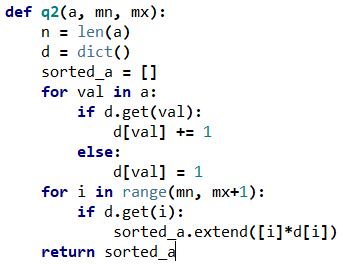
\includegraphics[width=0.8\textwidth]{q2.png}

\newpage
{\Large\bf Q3}\par
\textbf{(a)} There are $n-1$ comparisons done in the algorithm in the worst case.\par
\textbf{(b)} To extend this algorithm to find the second smallest element, use the method described to find the smallest element. Then, we know one of the elements beaten by the smallest is the second smallest, so we go back through each element that was compared to the smallest and return the smallest of those.\par
\textbf{(c)} There are $n-1$ comparisons done in the algorithm in the worst case to find the smallest element. The size of the array (n) passed to the function is divided by two each time until the array has 2 elements, which means there are $log_2(n)$ calls. We compare each element from these $log(n)$ calls compared to the smallest to find the second smallest. We ignore the one with the smallest since we know it's the smallest and don't need to compare it. This totals $log(n)-1$ comparisons. Adding all these comparisons yields $n+log(n)-2$ comparisons.
\end{document}